\chapter{Sistema embebido}

\section{Microcontroladores y/o microprocesadores utilizados}
En este proyecto, el microcontrolador LPC845 actúa como el núcleo de procesamiento central, manejando y coordinando la información que proviene de diversos sensores y periféricos. Este microcontrolador, basado en la arquitectura ARM Cortex-M0+, es seleccionado por su eficiencia energética y capacidad de realizar múltiples tareas de forma simultánea. A través de sus múltiples puertos de comunicación, el LPC845 se conecta con los componentes periféricos y transmite datos de estado directamente al Kinseal AMZ070W01RAGD, una pantalla que permite la visualización en tiempo real para el usuario. La interacción entre el LPC845 y el Kinseal es fundamental para la interfaz de usuario, ya que permite al operador monitorear el funcionamiento del sistema.

\section{Placas de desarrollo}
La placa de desarrollo empleada es la LPC845-BRK, una plataforma compacta que permite la rápida evaluación y desarrollo de aplicaciones basadas en el microcontrolador LPC845. La placa incluye una interfaz de depuración integrada, soporte para periféricos digitales y analógicos, y un puerto micro-USB para comunicación y programación. Este diseño compacto permite el acceso directo a los pines del microcontrolador, ideal para experimentación con módulos SPI y ADC. Esta configuración permite la conexión física con el Kinseal AMZ070W01RAGD, lo que facilita la implementación de la interfaz gráfica de usuario. Además, la placa proporciona estabilidad y protección a los circuitos, asegurando una transmisión de datos confiable entre el LPC845 y los periféricos.

\section{Software utilizados para el desarrollo}
El desarrollo de este sistema embebido se llevó a cabo con MCUXpresso IDE, un entorno de desarrollo integrado (IDE) específico para microcontroladores NXP. MCUXpresso proporciona herramientas avanzadas para depuración, control de periféricos y optimización de código en C/C++. Para la compilación y enlace del código, se empleó el compilador GNU ARM Toolchain compatible con la arquitectura Cortex-M0+. Además, se utilizó la biblioteca SDK de NXP que facilita la configuración de periféricos, manejo de GPIO, y control del módulo ADC y SPI. Además, para la configuración de la interfaz gráfica del Kinseal AMZ070W01RAGD, se emplearon los programas HMILite 2.22 y Kinseal Studio, diseñados para crear y gestionar interfaces HMI. HMILite 2.22 facilita la visualización en tiempo real de datos procesados, mientras que Kinseal Studio permite diseñar la interfaz gráfica que conecta al usuario con el sistema embebido.

\section{Diagrama en bloque de la solución}

    \begin{figure}[h]
        \centering
        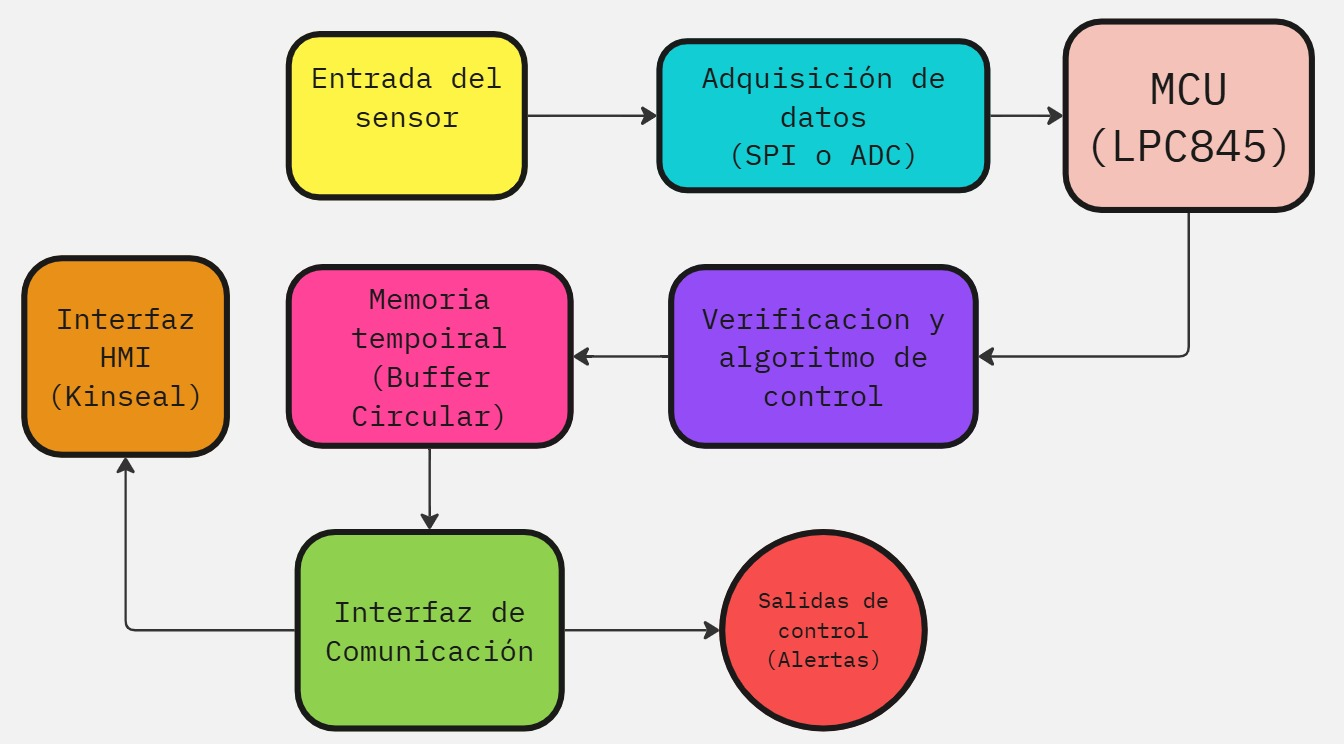
\includegraphics[width=0.8\textwidth]{Imagenes/Diagrama en bloques de sistema embibido.jpg}
        \caption{Diagrama en bloque de la solución}
        \label{fig:diagrama_bloque}
    \end{figure}

\section{Lenguajes de programación usados}
El sistema fue programado en C, un lenguaje de programación estructurado que es ampliamente utilizado en el desarrollo de sistemas embebidos por su eficiencia y control sobre el hardware. Las bibliotecas específicas de NXP permiten gestionar de manera eficiente los periféricos integrados, y el código está optimizado para la arquitectura ARM Cortex-M0+ del LPC845, garantizando un rendimiento adecuado en tiempo real. Para el desarrollo de la interfaz gráfica en el Kinseal AMZ070W01RAGD, Kinseal Studio permite el uso de un lenguaje de scripting específico para HMI, que facilita la creación de elementos gráficos y lógica de control en pantalla. Este lenguaje permite configurar la visualización de datos y ajustar la interactividad del sistema de manera personalizada, adaptándose a los requisitos del proyecto y logrando una interfaz amigable para el usuario.

\section{Especificación de periféricos utilizados}

\begin{itemize}
    \item \textbf{SPI (Serial Peripheral Interface):} Protocolo de comunicación utilizado para interactuar con el sensor de temperatura MAX6675. El SPI permite leer valores de temperatura en tiempo real y se configura con un reloj SCK de 1 MHz y distintos pines de selección de chip.
    
    \item \textbf{ADC (Analog-to-Digital Converter):} El sistema utiliza un ADC de 12 bits para leer valores analógicos de sensores de concentración de oxígeno, RPM y presión de aceite. Con un voltaje de referencia de 3.3V, el ADC convierte las señales analógicas en valores digitales, proporcionando precisión en la captura de datos del entorno.
    
    \item \textbf{GPIO (General-Purpose Input/Output):} Los pines GPIO permiten configurar salidas para el control de periféricos y selección de chips, activando y desactivando los pines CS de cada módulo.
\end{itemize}

\section{Estructuras de datos}

El sistema embebido utiliza una estructura de datos organizada y eficiente para almacenar, procesar y manejar la información recibida de los distintos sensores. Este diseño facilita el procesamiento en tiempo real, optimizando la memoria y permitiendo que el sistema mantenga datos consistentes y de fácil acceso. A continuación, se detallan las estructuras de datos utilizadas:

\subsection{Struct para sensores individuales}

Se define una estructura \texttt{SensorData} para cada sensor, que contiene campos específicos para cada medición. Esta estructura incluye los siguientes parámetros:

\begin{itemize}
    \item \texttt{float lectura}: valor de lectura convertido de datos analógicos a unidades físicas (°C para temperatura, rpm, bar para presión).
    \item \texttt{uint32\_t timestamp}: marca de tiempo para la toma de cada lectura, asegurando la sincronización en el procesamiento.
    \item \texttt{bool estado}: indicador de estado para verificar si la lectura es válida o si ha habido un error en el sensor.
\end{itemize}

\subsection{Especificación de periféricos utilizados}

En este sistema, los periféricos son esenciales para la adquisición y comunicación de datos críticos para el control del sistema embebido y su interfaz gráfica con el usuario. A continuación, se detallan los periféricos clave utilizados:

\begin{itemize}
    \item \textbf{MAX6675}: Este sensor se utiliza para medir la temperatura en las termocuplas de cabeza de cilindro. Proporciona datos de temperatura precisos y confiables mediante la interfaz SPI, lo que permite un monitoreo efectivo de las condiciones térmicas del motor.
    
    \item \textbf{MAX31865}: Se utiliza para los termistores de aceite y de agua. Este conversor RTD convierte la resistencia del termistor a una lectura digital precisa, proporcionando datos de alta precisión para el monitoreo de la temperatura del aceite y del agua en el sistema. La comunicación con el LPC845 se realiza a través de la interfaz SPI.

    \item \textbf{Sensor de presión de aceite}: Este sensor mide la presión en el sistema de aceite, proporcionando información esencial para el monitoreo del motor. La comunicación se realiza a través de la entrada ADC del LPC845.

    \item \textbf{Sensor de concentración de oxígeno}: Captura los niveles de oxígeno y se comunica con el microcontrolador para ofrecer datos críticos sobre la combustión y otros parámetros ambientales. Este sensor también se conecta mediante la interfaz ADC.

    \item \textbf{Sensor de RPM}: Este sensor permite la lectura de la velocidad del motor en revoluciones por minuto (RPM). Utiliza la entrada ADC del LPC845 para medir la señal analógica proporcional a la velocidad del motor, proporcionando lecturas en tiempo real. Esta configuración garantiza una alta precisión en el monitoreo de RPM y permite ajustar la respuesta del sistema en función de la velocidad del motor.

    \item \textbf{Comunicación con Kinseal AMZ070W01RAGD}: La pantalla táctil Kinseal está conectada al sistema mediante comunicación serial UART. A través de este canal, el LPC845 envía información de cada sensor y recibe comandos, actualizando en tiempo real la interfaz gráfica desarrollada en Kinseal Studio con el software HMILite 2.22.
\end{itemize}

Esta combinación de periféricos asegura que el sistema embebido capture, procese y comunique los datos relevantes, permitiendo una visualización y control eficientes en el dispositivo HMI.
